\chapter{A Methodology to Evaluate PX in Rehabilitation Exergames}
\label{ch:methodology}
%%% Introduction (Explain and contextualise objective)
%After proposing a PX Model, evaluators will benefit having a methodology that guides them in the process of planning, executing, analysing and reporting an evaluation. This, methodology also guides on how to use the model for evaluation purposes.
We presented some constraints that evaluators should consider when evaluating \ac{PX} in rehabilitation exergames in \autoref{ch:characterising}. Additionally, we identified the importance of selecting evaluation aspects, methods and instruments purposely. As presented in \autoref{ch:model}, depending on the layer of abstraction and the moment being assessed, different aspects may be relevant; e.g., rehabilitation aspects are relevant to evaluate progress after one or several episodes of gameplay. In this section, we present a methodology that attempts to guide evaluators through the process of selecting evaluation aspects, methods and instruments to assess \ac{PX} in rehabilitation exergames. This methodology is intended to be used along the whole development life cycle. It can be used iteratively refining the outcomes/decisions of each stage after each iteration. If a rehabilitation exergame is a collection of mini-games, each mini-game should be evaluated separately. The stages of our methodology are illustrated in \autoref{fig:PXEvaluationMethodology} and detailed below.

\begin{figure}[bth]
\myfloatalign
{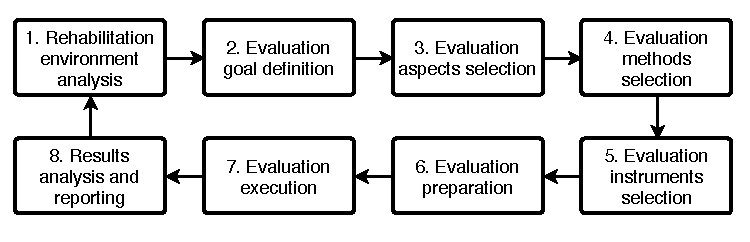
\includegraphics[width=\linewidth]{gfx/methodology/PXEvaluationMethodology}} \quad
\caption{Stages of the proposed methodology}\label{fig:PXEvaluationMethodology}
\end{figure}

%PX evaluations methodologies, %How digital games for rehabilitation have been evaluated
% RioOlarte-- check paper annotations

%Materials and Methods
%Results from previous chapter????


\section{Rehabilitation environment}
Evaluators should characterise players to identify the needs to be considered during evaluation. To achieve this, they can use methods such as ethnography, cultural debugging, player modelling, interview and focus groups. Then, evaluators should identify additional evaluation constraints; e.g., those imposed by regulations and internal processes of the health institution where evaluation may occur. Evaluators should concentrate on the logistics that are required to perform an evaluation, e.g., participants, location, regulations, etc. When a rehabilitation exergame consists of collection of mini-games, each mini-game should be separately characterised. Below, we present an approach to characterise a rehabilitation exergame.

\subsection{Characterising rehabilitation exergames}
To characterise a rehabilitation exergame, we need a set of properties that allow understanding its role within a physical therapy. Evaluators can use the approach presented in \autoref{sec:characterising} to characterise the rehabilitation exergame to be evaluated.

\subsection{Evaluation goal definition}
Evaluators should now define the evaluation goal based on the development maturity of the exergame. First, evaluators should focus on assuring patient’s safety. Then, effectiveness and common \ac{PX} aspects can be evaluated. 

\subsection{Evaluation aspects selection}
Selecting the aspects to be evaluated is a crucial task to be overcome when preparing an evaluation. This selection depends on aspects such as evaluation goal, available resources, development maturity of the evaluated rehabilitation exergame and the \ac{PX} moment being evaluated. A discussion about relevant aspects to evaluate in rehabilitation exergames was presented in \autoref{sec:rehab_aspects}. Also, \autoref{tab:aspectsModelMappingContext}, \autoref{tab:aspectsModelMappingPlayer} and \autoref{tab:aspectsModelMappingGame} present the aspects to be evaluated during each moment of \ac{PX} for the context, the player/patient and the game system layers of abstraction respectively.

\begin{table}[h]
\caption{Aspects to evaluate for the context layer over time}
\label{tab:aspectsModelMappingContext}
\begin{center}
\begin{tabularx}{\textwidth}{p{6cm}XXp{2cm}}
\toprule
\multirow{2}{*}{\spacedlowsmallcaps{Aspect}} & \multicolumn{3}{c}{\spacedlowsmallcaps{Moment of PX}} \\
\cline{2-4}
 & \spacedlowsmallcaps{Antecedents} & \spacedlowsmallcaps{Interaction} & \spacedlowsmallcaps{Effects} \\
\midrule
Physiotherapists preference & X &  &  \\
\midrule
Physiotherapists expectations & X &  &  \\
\midrule
Game diffusion & X &  &  \\
\midrule
Location & X & X &  \\
\midrule
Competence &  & X &  \\
\midrule
Collaboration &  & X &  \\
\midrule
Game knowledge generation &  &  & X \\
\midrule
Institutions regulations/processes & X &  &\\
\midrule
\bottomrule
\end{tabularx}
\end{center}
\end{table}

\begin{table}[h]
\caption{Aspects to evaluate for the player/patient layer over time}
\label{tab:aspectsModelMappingPlayer}
\begin{center}
\begin{tabularx}{\textwidth}{p{6cm}XXp{2cm}}
\toprule
\multirow{2}{*}{\spacedlowsmallcaps{Aspect}} & \multicolumn{3}{c}{\spacedlowsmallcaps{Moment of PX}} \\
\cline{2-4}
 & \spacedlowsmallcaps{Antecedents} & \spacedlowsmallcaps{Interaction} & \spacedlowsmallcaps{Effects} \\
\midrule
Challenge, flow &  & X &  \\ \midrule
Emotion & X & X & X \\ \midrule
Engagement &  & X &  \\ \midrule
Negative-positive affect &  & X & X \\ \midrule
Enjoyment, fun &  & X &  \\ \midrule
Immersion, absorption, presence &  & X &  \\ \midrule
Attention &  & X &  \\ \midrule
Interest & X &  & X \\ \midrule
Story & X & X &  \\ \midrule
Tension &  & X &  \\ \midrule
Aesthetics &  & X &  \\ \midrule
Curiosity &  & X &  \\ \midrule
Accomplishment &  & X & X \\ \midrule
Clarity of game goals &  & X &  \\ \midrule
Ease of use &  & X &  \\ \midrule
Cognitive load &  & X &  \\ \midrule
Learnability &  & X &  \\ \midrule
Preference & X &  & X \\ \midrule
Rehabilitation goal achievement &  &  & X \\ \midrule
Physical rehabilitation aspects & X & X* & X \\ \midrule
Movement meaningfulness & X &  &  \\ \midrule
Tutorial understanding &  & X &  \\
\midrule
\bottomrule
\end{tabularx}
* If supported by the rehabilitation exergame or other equipment
\end{center}
\end{table}

\begin{table}[htb]
\caption{Aspects to evaluate for the game system layer over time}
\label{tab:aspectsModelMappingGame}
\begin{center}
\begin{tabularx}{\textwidth}{p{6cm}XXp{2cm}}
\toprule
\multirow{2}{*}{\spacedlowsmallcaps{Aspect}} & \multicolumn{3}{c}{\spacedlowsmallcaps{Moment of PX}} \\
\cline{2-4}
 & \spacedlowsmallcaps{Antecedents} & \spacedlowsmallcaps{Interaction} & \spacedlowsmallcaps{Effects} \\
\midrule
Playability & X & X & X \\ \midrule
Functionality & X & X &  \\ \midrule
Configuration capability & X &  &  \\ \midrule
Adaption capability &  & X &  \\ \midrule
Movement mapping correctness & X &  &  \\ \midrule
Movement mapping completeness & X &  &  \\ \midrule
Monitoring &  & X &  \\ \midrule
Movement correction &  & X &  \\ \midrule
Movement correctness feedback &  & X &  \\ \midrule
Progress feedback &  & X & X \\ \midrule
Tutorial completeness & X &  &  \\ \midrule
Point of view &  & X &  \\ \midrule
\bottomrule
\end{tabularx}
\end{center}
\end{table}


\subsection{Evaluation methods selection}
Evaluators should select methods based on the selected aspects and available re-sources; e.g., experts, participants, location and evaluation instruments. A discussion about relevant methods to evaluate in rehabilitation exergames was presented in \autoref{sec:rehab_methods}. Moreover,  \autoref{tab:methodsModelMappingPlayer}, \autoref{tab:methodsModelMappingContext} and \autoref{tab:methodsModelMappingGame} present the methods that evaluators can use to assess the context, the player/patient and the game system layers of abstraction respectively, during each moment of \ac{PX}.

\begin{table}[h]
\caption{Evaluation methods for the player/patient layer over time}
\label{tab:methodsModelMappingPlayer}
\begin{center}
\begin{tabularx}{\textwidth}{p{6cm}XXp{2cm}}
\toprule
\multirow{2}{*}{\spacedlowsmallcaps{Method}} & \multicolumn{3}{c}{\spacedlowsmallcaps{Moment of PX}} \\
\cline{2-4}
 & \spacedlowsmallcaps{Antecedents} & \spacedlowsmallcaps{Interaction} & \spacedlowsmallcaps{Effects} \\
\midrule
Questionnaires & X & X & X \\ \midrule
Interview & X &  & X \\ \midrule
Video recording &  & X &  \\ \midrule
Field-Behavioural observation & X & X & X \\ \midrule
Think-aloud protocol &  & X &  \\ \midrule
Focus groups & X & X & X \\ \midrule
Question-asking protocol &  & X &  \\ \midrule
Biometrics analyse & X &  & X \\ \midrule
\ac{EEG}, \ac{EMG}, \ac{EDA}, \ac{HR} & X & X & X \\ \midrule
Body movement coding &  & X &  \\ \midrule
Eye-tracking &  & X &  \\ \midrule
Persona modelling & X &  &  \\ \midrule
Player modelling & X &  &  \\ \midrule
Physical rehabilitation tests & X &  & X \\ \midrule
Physiotherapist observation & X & X & X \\ \midrule
\bottomrule
\end{tabularx}
\end{center}
\end{table}

\begin{table}[htb]
\caption{Evaluation methods for the context layer over time}
\label{tab:methodsModelMappingContext}
\begin{center}
\begin{tabularx}{\textwidth}{p{6cm}XXp{2cm}}
\toprule
\multirow{2}{*}{\spacedlowsmallcaps{Method}} & \multicolumn{3}{c}{\spacedlowsmallcaps{Moment of PX}} \\
\cline{2-4}
 & \spacedlowsmallcaps{Antecedents} & \spacedlowsmallcaps{Interaction} & \spacedlowsmallcaps{Effects} \\
\midrule
Questionnaires & X & X & X \\ \midrule
Interview & X &  & X \\ \midrule
Field-Behavioural observation & X & X &  \\ \midrule
Focus groups & X &  & X \\ \midrule
Co-discovery learning &  & X &  \\ \midrule
Peer tutoring &  & X &  \\ \midrule
Prisoner dilemma task &  & X &  \\ \midrule
Ethnography & X & X & X \\ \midrule
Cultural debugging & X &  &  \\ \midrule
\bottomrule
\end{tabularx}
\end{center}
\end{table}

\begin{table}[htb]
\caption{Evaluation methods for the game system layer over time}
\label{tab:methodsModelMappingGame}
\begin{center}
\begin{tabularx}{\textwidth}{p{6cm}XXp{2cm}}
\toprule
\multirow{2}{*}{\spacedlowsmallcaps{Method}} & \multicolumn{3}{c}{\spacedlowsmallcaps{Moment of PX}} \\
\cline{2-4}
 & \spacedlowsmallcaps{Antecedents} & \spacedlowsmallcaps{Interaction} & \spacedlowsmallcaps{Effects} \\
\midrule
\ac{RITE} & X & X &  \\ \midrule
Heuristic evaluation & X & X & X \\ \midrule
Guidelines or standard inspections & X & X & X \\ \midrule
Cognitive walkthrough & X & X & X \\ \midrule
Pluralistic walkthrough & X & X & X \\ \midrule
Gameplay metrics &  & X &  \\ \midrule
Game logs &  & X &  \\ \midrule
A/B Testing & X & X & X \\ \midrule
\bottomrule
\end{tabularx}
\end{center}
\end{table}

\subsection{Evaluation instruments selection}
Evaluators should select evaluation instruments based on the aspects and methods involved in the evaluation. Evaluation instruments for rehabilitation exergames may be borrowed from \ac{GUR}, \ac{UX} and physical rehabilitation fields. A discussion about relevant instruments to evaluate in rehabilitation exergames was presented in \autoref{sec:rehab_instruments}.

\subsection{Evaluation preparation}
Evaluators should prepare all logistics associated to evaluation. They should prepare a test protocol based on the outcomes of the previous stages.

\subsection{Evaluation execution}
Researchers conduct planned evaluation. The evaluation may occur in a laboratory, at a health institution or even at a house.

\subsection{Results analysis and reporting}
Evaluators analyse the data collected during evaluation and reports findings and recommendations considering the evaluation goal. This is a common task on usability and UX evaluation, thus, similar approaches can be employed.


%%%%Results and discussion - Methodology

% Antecedents in proposed model
%An iterative methodology composed of a set of stages that considers rehabilitation constraints


% stages, check paper


%table mapping methods, instruments, aspects???


%Ideas in progress...
%%%Conclusions and recommendations for the objective
% check paper

\section{PX evaluation web application}
A web application to manage \ac{PX} evaluations was developed using the Django framework \footnote{Django Project: \url{www.djangoproject.com}} (See \autoref{fig:dashboardApp}). The application contains ten modules that allow registering, updating and listing \ac{PX} evaluations for rehabilitation exergames following the methodology presented in this chapter. The \autoref{fig:evaluationApp1} present the view of an evaluation being registered at the application and \autoref{fig:evaluationApp2} presents its detail view. To aim that, the following features are available:

\begin{enumerate}
    \item Registering, updating and listing evaluation aspects.
    \item Registering, updating and listing evaluation methods.
    \item Registering, updating and listing evaluation instruments.
    \item Registering, updating and listing evaluation questionnaires, following the standard presented in \autoref{ch:questionnaire} (See \autoref{fig:standardApp}).
    \item Registering, updating and listing rehabilitation exergames following the characterising approach presented in \autoref{sec:characterising} (See \autoref{fig:characterisingApp}).
    \item Registering, updating and listing rehabilitation constraints.
    \item Registering, updating and listing rehabilitation associated tasks (e.g, supervising and motivating).
    \item Registering, updating and listing interaction devices and technologies.
    \item Registering, updating and listing rehabilitation movements and configuration parameters.
    \item Registering, updating and listing pathologies.
    \item Registering, updating and listing resources (e.g. evaluation reports or protocols).
    \item A wiki to access to articles explaining the \ac{PX} evaluation methodology and the questionnaire standard.
\end{enumerate}

The application was developed using agile practices such as the use of a task-board, user stories and issues. The development process was managed using the ZenHub\footnote{https://www.zenhub.com/} application and the code versioning was managed using git\footnote{https://git-scm.com/} and GitHub\footnote{https://github.com/}. The source code of the application is available at \url{https://github.com/edwingamboa/rehab-exergames-px-app}.

\begin{figure}[bth]
\myfloatalign
{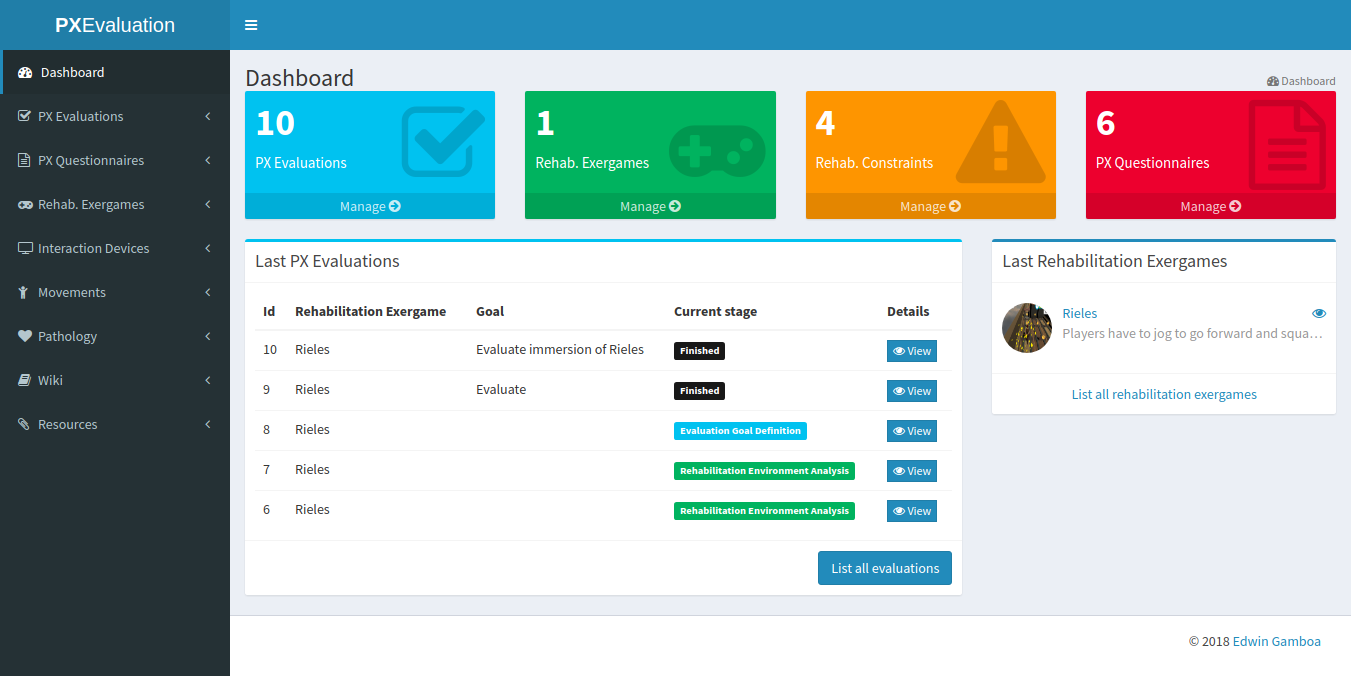
\includegraphics[width=\linewidth]{gfx/app/dashboardApp}} \quad
\caption{Dashboard of the \ac{PX} evaluation application}\label{fig:dashboardApp}
\end{figure}

\begin{figure}[bth]
\myfloatalign
{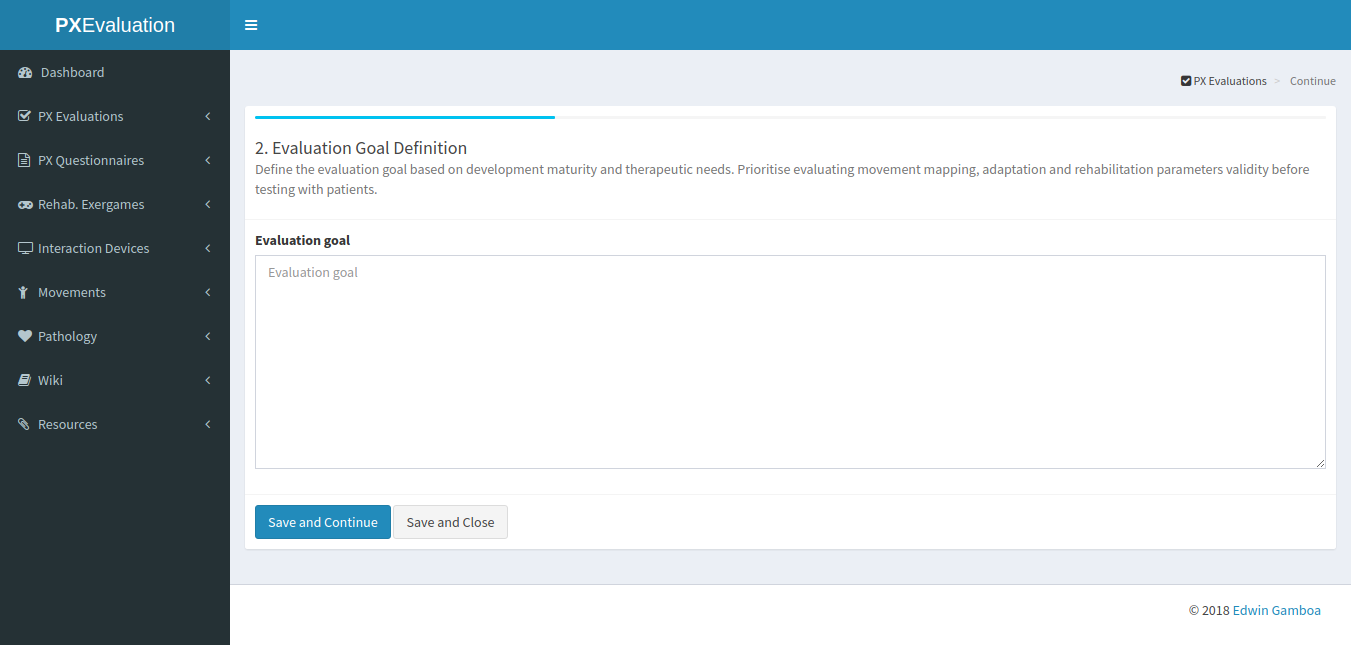
\includegraphics[width=\linewidth]{gfx/app/evaluationApp1}} \quad
\caption{Register view of an evaluation at the \ac{PX} evaluation application}\label{fig:evaluationApp1}
\end{figure}

\begin{figure}[bth]
\myfloatalign
{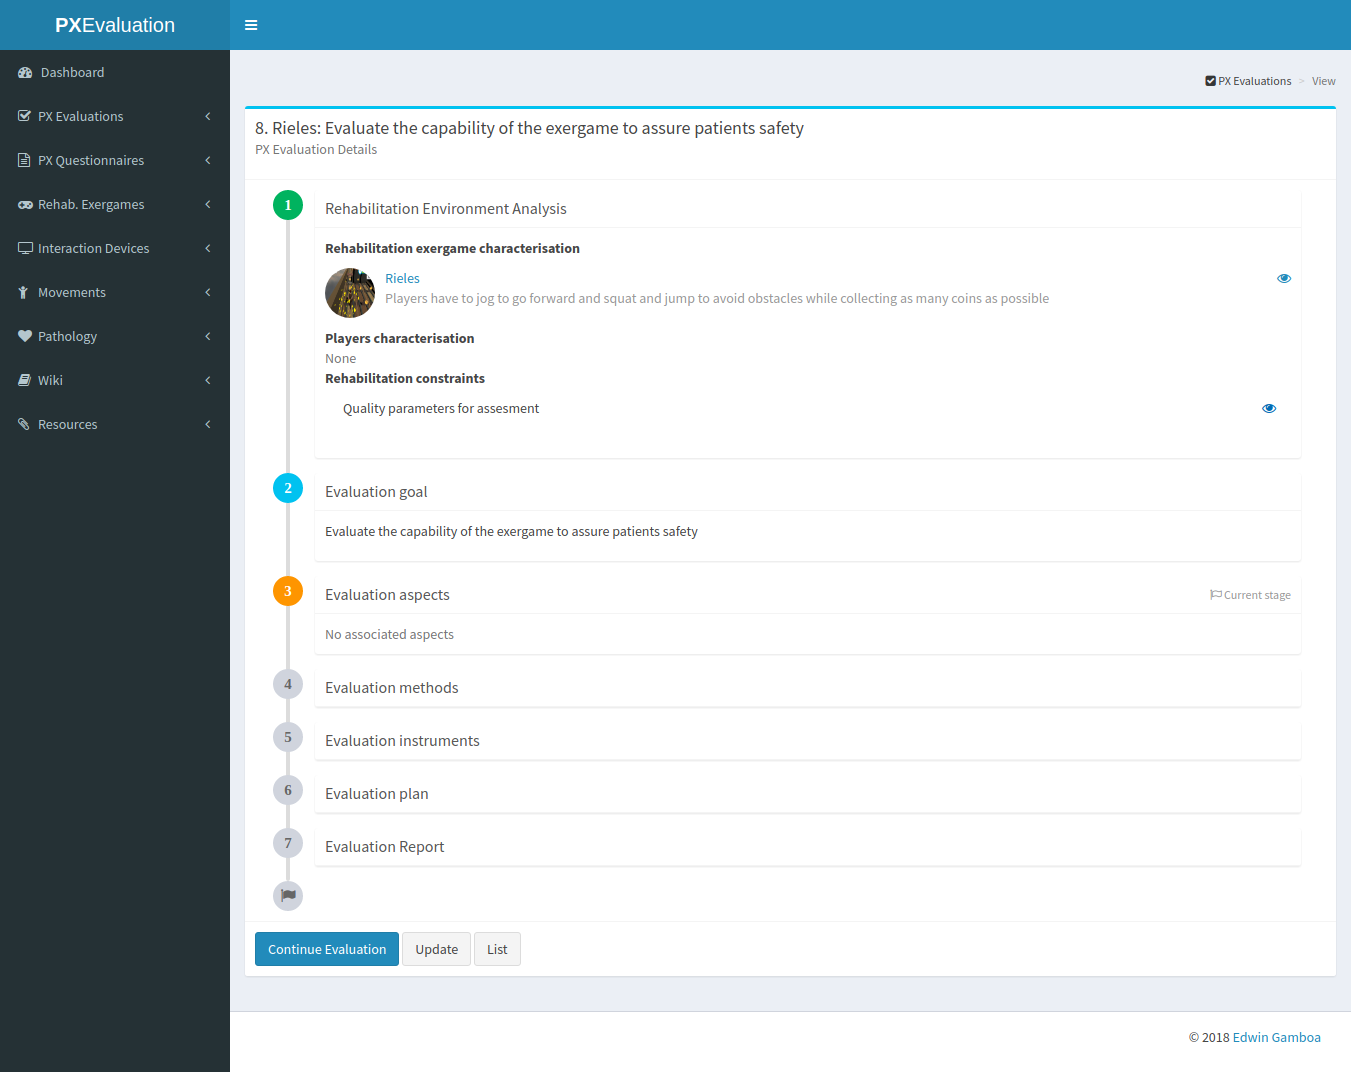
\includegraphics[width=\linewidth]{gfx/app/evaluationApp2}} \quad
\caption{Detail view of an evaluation at the \ac{PX} evaluation application}\label{fig:evaluationApp2}
\end{figure}


\begin{figure}[bth]
\myfloatalign
{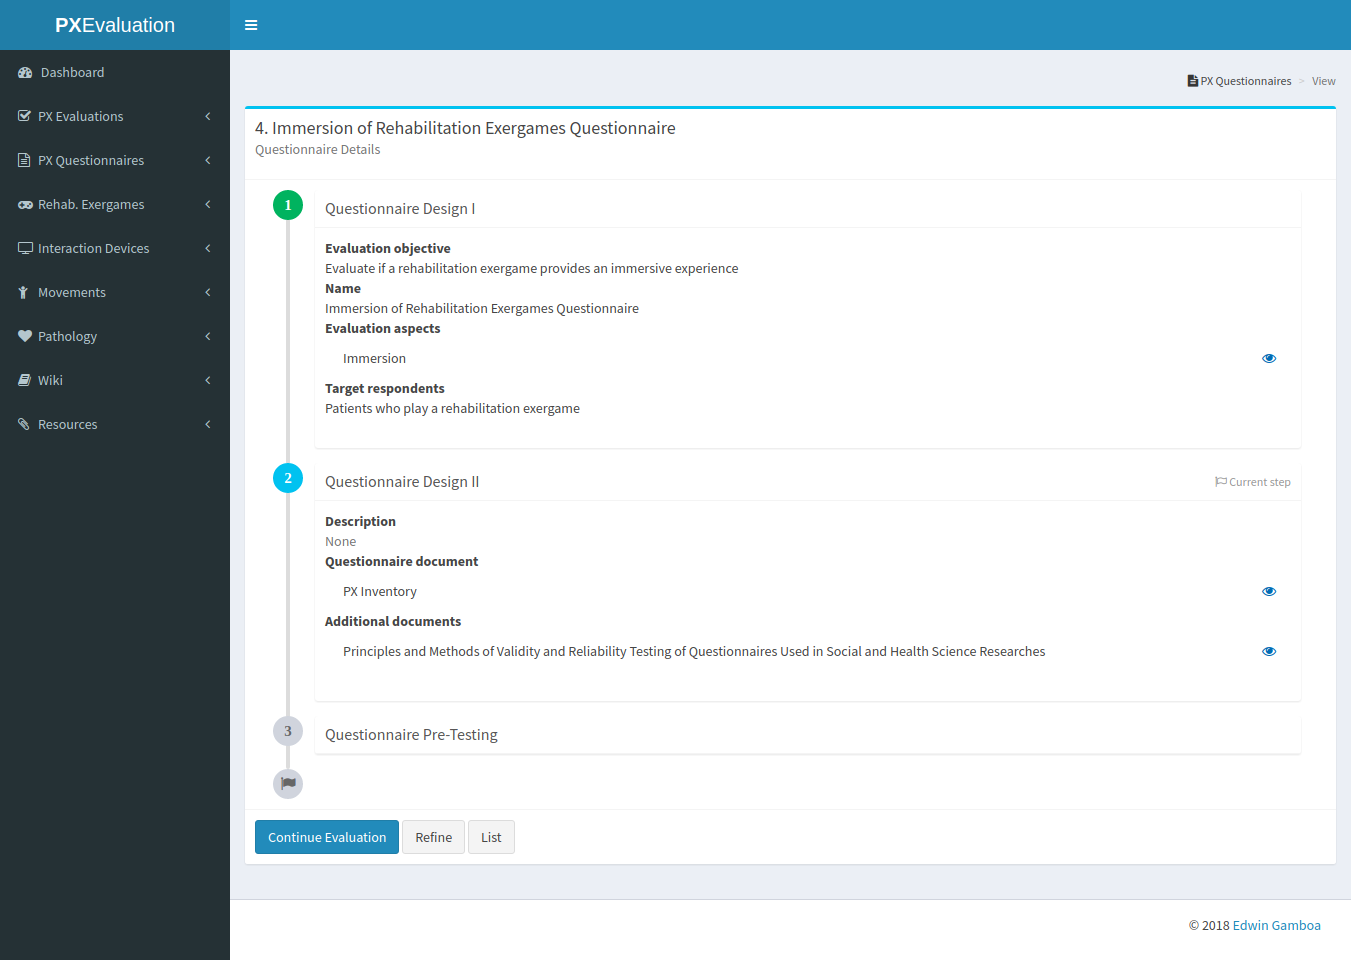
\includegraphics[width=\linewidth]{gfx/app/standardApp}} \quad
\caption{Detail view of a standard being developed at the \ac{PX} evaluation application}\label{fig:standardApp}
\end{figure}

\begin{figure}[bth]
\myfloatalign
{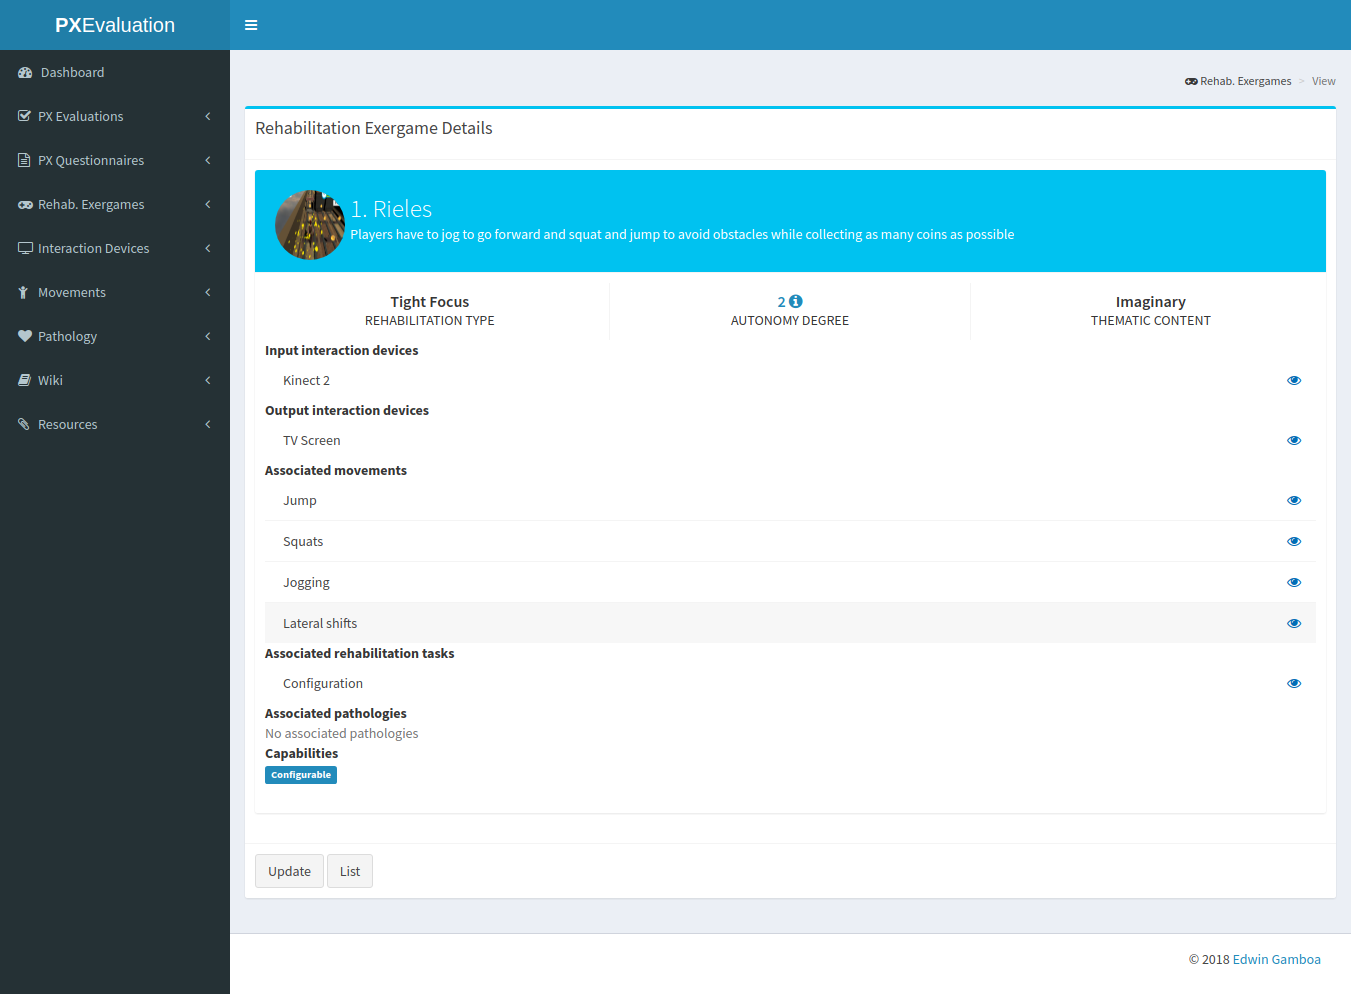
\includegraphics[width=\linewidth]{gfx/app/characterisingApp}} \quad
\caption{Detail view of a rehabilitation exergame characterisation at the \ac{PX} evaluation application}\label{fig:characterisingApp}
\end{figure}

\clearpage
\section{Conclusion}
In this chapter, we presented a methodology for evaluating PX in rehabilitation exergames. Our proposal is based on the model presented on \autoref{ch:model}; highlighting crucial aspects to be evaluated before, during and after interaction between a patient, a context and a rehabilitation exergame occurs. Since the methodology is based on a \ac{PX} model for rehabilitation exergames, it allows performing evaluations that meet the constraints that the rehabilitation environment may impose. It requires evaluators to characterise rehabilitation exergames considering its therapeutic goal, to define users profile considering its characteristics as patients and analysing the involved rehabilitation environment. Thus, our approach differs from other evaluations in which exergames are evaluated considering only motivation, enjoyment or usability \autocite{Brokaw2015,Burke2009,Cameirao2010,jansen2013serious,Ni2014}.

The proposed methodology is intended to be used iteratively to perform a comprehensive evaluation. However, it was built based on a model designed using a qualitative approach, thereby limiting its generalisation. Thus, we still need to use the methodology extensively to identify gaps and additional constraints that should be considered. This process would allow us to validate the relevance of the highlighted stages in real use cases.

Finally, the proposed methodology may be extended or adapted to other domains in which entertainment is not the main goal. In that case, the domain constraints should be identified to define a set of relevant aspects, methods and instruments to be employed during \ac{PX} evaluation.
